\chapter{High throughput generation of genetic markers}
\thispagestyle{empty}
\label{chap:pheno2geno}
\emph{Using prior knowledge about phenotypes and how they are transfered during 
reproduction allows us to create phenotype based genetic markers. We can use 
these derived markers to saturate existing genetic maps or create them de-novo 
when enough data is available. Pheno2Geno was developed to use a sensitive 
pre-selection and mixture modeling approach to improve performance. The package 
is designed to be fast enough to make use of data from diverse data sources such 
as: microarrays, tiling arrays and/or RNA-Seq experiments. Using data from tiling 
arrays we were able to improve the genetic map resolution of an A. thaliana 
Recombinant Inbred Line (RIL) derived from a Bayreuth (Bay-0) x Shahdara (Sha) cross.}

\null
\vfill

\begin{myexampleblock}{Under review:}
  \authors{Konrad Zych*, K. Joeri van der Velde, Ronny V. L. Joosen, Wilco Ligterink, Ritsert C Jansen and Danny Arends}\\
  \emph{Pheno2Geno - High throughput generation of genetic markers and maps from molecular phenotypes}\\
  \bold{BMC Bioinformatics} (XXXX)
\end{myexampleblock}
\newpage

\section{Pheno2Geno}
Genetic markers and maps are instrumental for quantitative trait locus (QTL) mapping in segregating 
populations. The resolution of QTL localisation depends on the number of informative recombinations 
in the population and how well these recombinations are tagged by markers. Thus larger populations 
and denser marker maps perform better at detecting and locating QTLs. In practice, marker maps are 
often still too sparse. However, maps can be saturated or even be derived \emph{de-novo} from high-
throughput omics data, such as gene expression, protein or metabolite abundance data. This is because 
molecular phenotypes are influenced by genetic variation and they will show a clear multimodal 
distribution due to major QTL effects, such information can therefore be converted into useful 
genetic markers.

The Pheno2Geno R package is developed for high-throughput generation of genetic markers and maps from 
molecular phenotypes. Pheno2Geno selects suitable phenotypes that show clear differential expression 
in the founders. Pheno2Geno uses mixture modeling to select phenotypes showing segregation ratios 
close to the expected mendelian segregation ratios and transform them into genetic markers suitable 
for map construction and/or saturation. Pheno2Geno analyses the candidate genetic markers and excludes 
those showing multiple QTL, epistatically interacting QTL, and QTL by environment interactions to 
provide a set of robust markers for QTL mapping protecting against genetic markers from a non genetic 
origin.

We demonstrate our tool using gene expression data of 370.000 transcripts in 164 \emph{A. thaliana} 
Recombinant Inbred Lines (RILs). Pheno2Geno is able to saturate the existing genetic map decreasing 
the average distance between markers from 7.1 cM to 0.89 cM, close to the theoretical limit of 0.6 cM, 
pinpointing almost all of the informative recombinations in the population. Pheno2Geno is also able 
to created a \emph{de-novo} map from the gene expression data that is twice as dense as the original 
genetic map.

The Pheno2Geno package offers high-throughput \emph{de-novo} map construction and saturation of 
existing genetic maps. Processing of the showcase dataset takes less than 30 minutes on an average 
desktop PC. Pheno2Geno improves QTL mapping results at no additional laboratory cost and with 
minimum computational effort. Pheno2Geno results are formatted for direct use in R/qtl, the leading 
R package for QTL studies. Pheno2Geno is freely available on CRAN under GNU GPL version 3.

\section{Background}
QTL mapping \cite{Lander:1989} is a powerful approach used in population analysis to link 
genetic variation to phenotypic variation. It requires polymorphic genetic markers positioned 
on a genetic map. Phenotypes showing a dichotome 0/1 distribution with approximate equal 
proportions in, say, a RIL population can be used as genetic markers: genotypes can be 
called by connecting the 0/1 to the parental strains A/B. Such markers can then be used 
for de-novo construction of the genetic map or for saturation of a known genetic map 
\cite{West:2006, Truco:2013}.

Continuous (non-dichotome) phenotypes can also be used as markers if they show a major QTL: a 
major QTL will cause the phenotype to show a clear multimodal distribution to which a mixture 
models can be fitted \cite{Jansen:1993, Jansen:2001a}. Posterior probabilities derived from 
mixture modeling are used for genotype calling. Such approaches have been used for up to 
1,200 molecular phenotypes \cite{Gort:2010}.

Here, we scale up the mixture model approach for non dichotome phenotypes in order to make 
analysis of hundreds of thousands of molecular phenotypes feasible e.g. gene expression data.

Genetic maps created by Pheno2Geno can be easily used for QTL mapping: the package provides 
output structures compatible with R/qtl, the leading R package for QTL analysis in 
experimental crosses \cite{Broman:2003, Arends:2010}. Pheno2Geno allows users to 
explore and compare resulting maps with their favorite genome browser. Maps can be saved
as a GFF (General Feature Format) file that is supported by most genome browsers.

\begin{figure}[h!]
  \centering
  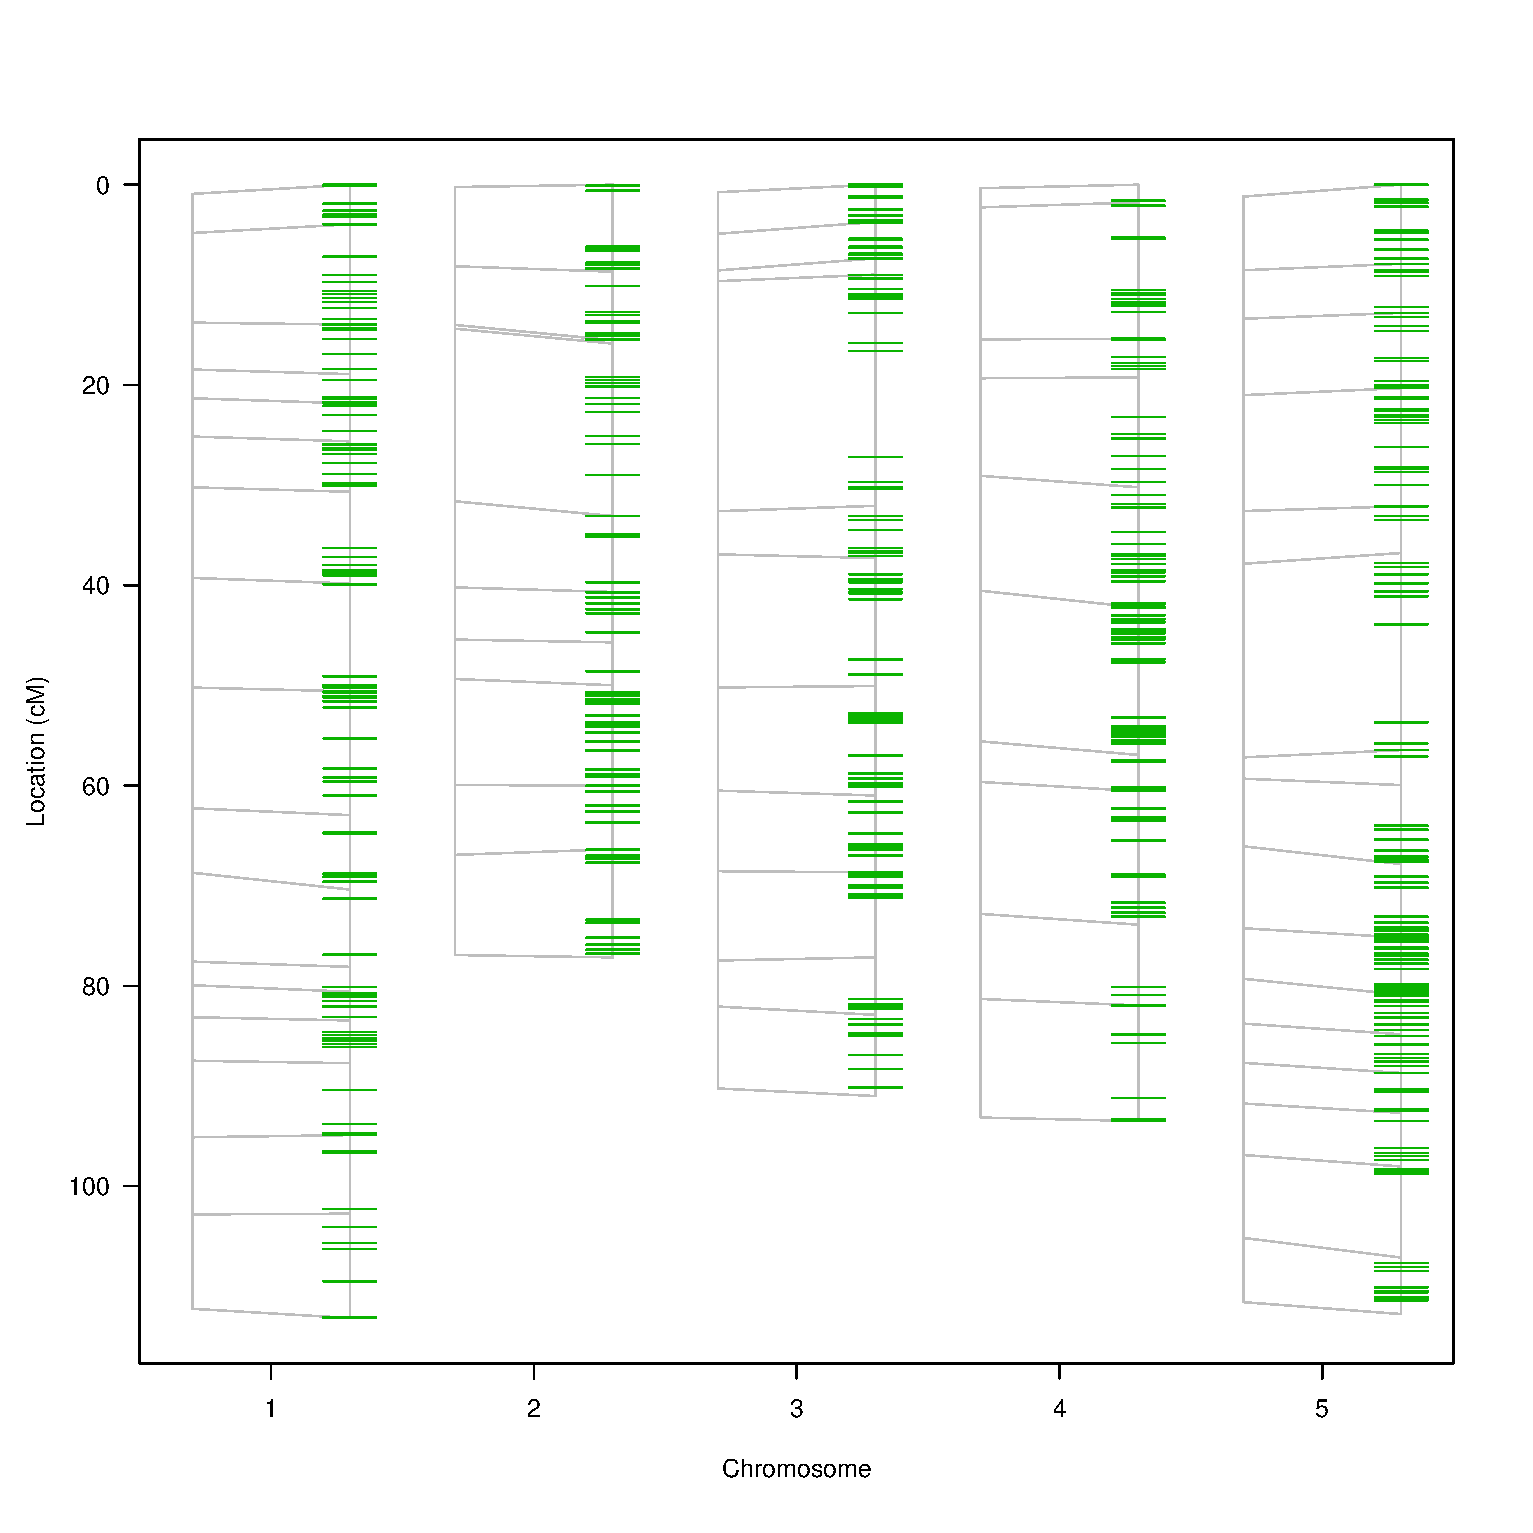
\includegraphics[keepaspectratio,width=0.8\textwidth]{eps/image_2_1.eps}
  \caption[Map comparison]{Map comparison plot drawn using R/qtl function \emph{plot.map} \cite{Broman:2003, Arends:2010}. For 
          each of the chromosomes the original map (left) and the saturated map (right) are plotted. Lines are drawn
          to connect markers.  Markers that exist in just one map and not the other are indicated by short line 
          segments, on one side or the other, that are not connected across. Before plotting, both maps were 
          re-estimated using the R/qtl function \emph{est.map}. The original map consists of 5 chromosomes and 69 
          markers at an average distance of 7.1 cM. The saturated map consists of the original 69 markers plus 497 
          expression-based markers at an average marker distance of 0.89 cM.}
          s\label{fig:mapcomparison}
\end{figure}

\begin{figure}[h!]
  \centering
  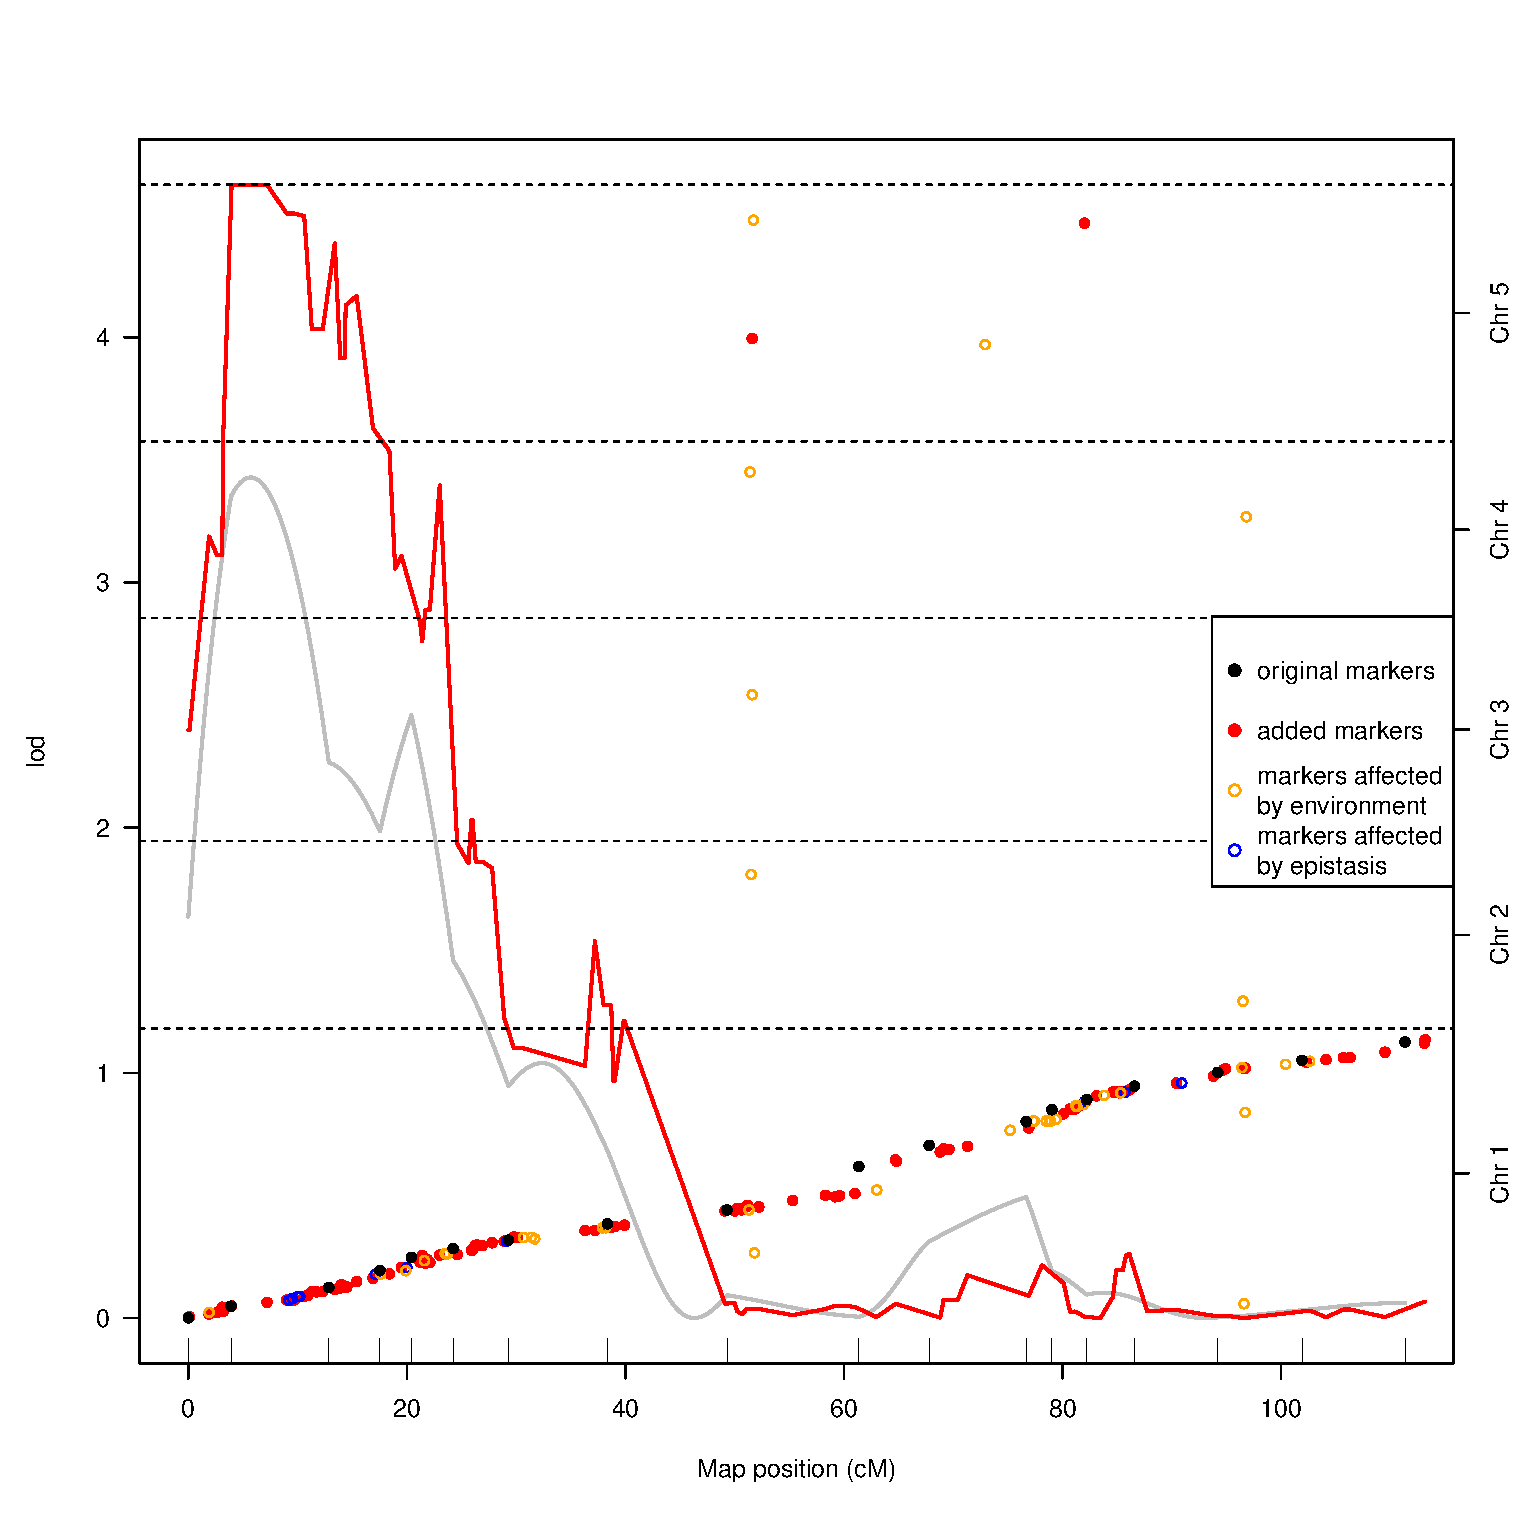
\includegraphics[keepaspectratio,width=0.8\textwidth]{eps/image_2_2.eps}
  \caption[single-marker QTL mapping]{Results of single-marker QTL mapping of a classical phenotype on original (gray line) and saturated map (green line)(left axis). 
          Only chromosome 1 is shown.
          {\bf Ticks on an X-axis} - positions of the original markers on the genetic map. 
          {\bf Gray dots} - positions of the original markers on the physical map. 
          {\bf Colored dots and circles} - candidate markers detected by Pheno2Geno.
          {\bf Orange circles} - candidate markers removed because they showed significant environmental influence.
          {\bf Red circles} - candidate markers removed because they showed an epistatic interaction with other genetic markers. 
          {\bf Green dots} - markers used for saturation of the original map. 
          The final saturated map consists of all the green and gray dots. Shown here are locations of the new markers on the old map, in 
          this way maps align for better clarity.}
          \label{fig:qtlcomparison}
\end{figure}

\begin{figure}[h!]
  \centering
  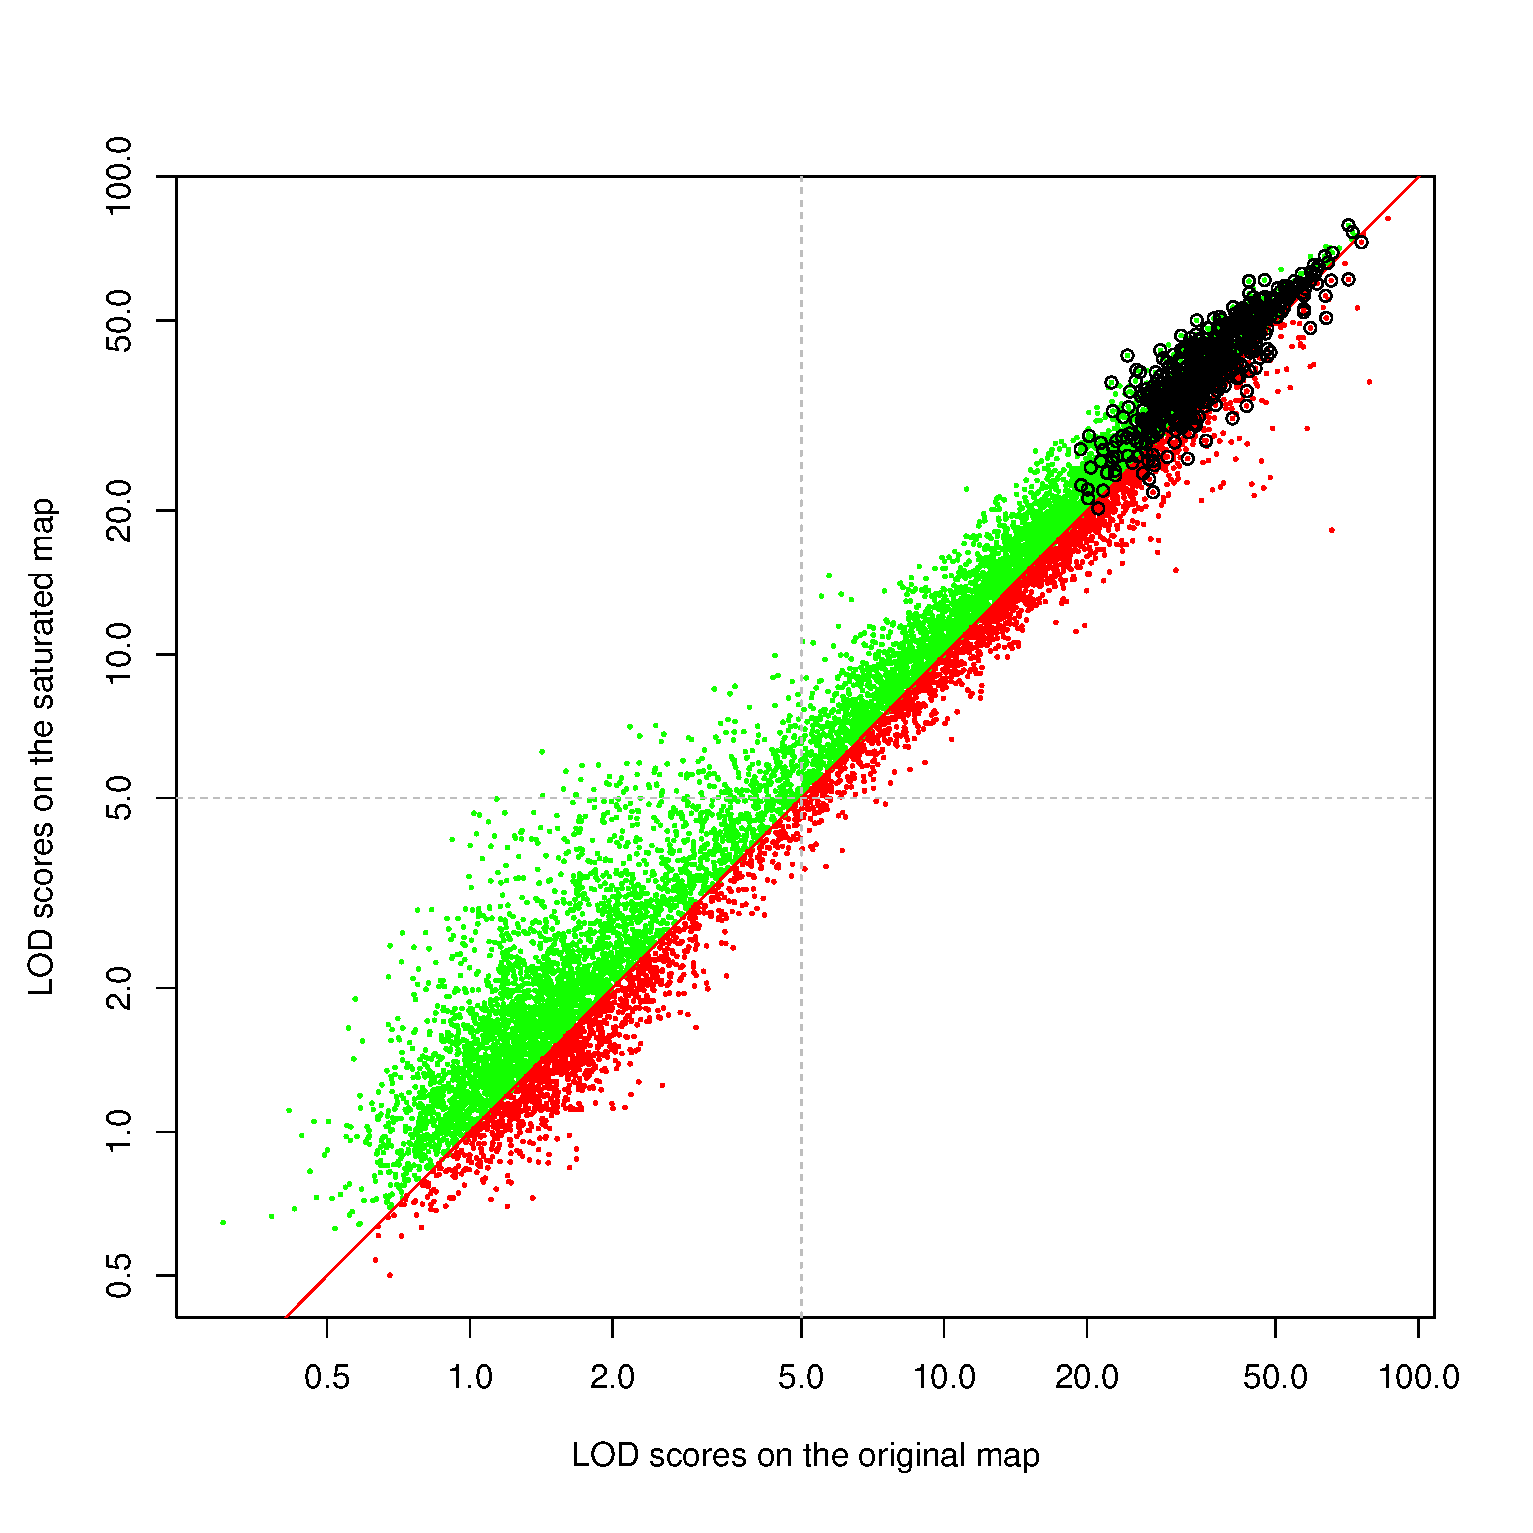
\includegraphics[keepaspectratio,width=0.8\textwidth]{eps/image_2_3.eps}
  \caption[LOD changes.]{
          {\bf A) LOD scores on original and saturated map}. QTL mapping was performed on all 10,801 SNP probes showing differential 
          expression between parents ($p < 0.01$ Student t-test) using original and saturated map. 5837 probes show   a QTL with a 
          $LOD > 5$ on  the original map. {\bf Blue dots} - 3943 probes (66\%) that show an increased LOD score on the new saturated map. 
          Moreover, 210 new QTLs were detected on the saturated map. 
            {\bf Red dots} -  probes showing a decrease in LOD score on the saturated map. 
            {\bf Green circles} - probes used to saturate the map.
          {\bf B) Changing LOD scores.} For each of the phenotypes the top QTL  peak was selected. If the peaks measured on original 
          and saturated map shared location, the differences between LOD scores was calculated. {\bf Solid green line} - median of 
          differences between peaks from chromosome 4, calculated inside a sliding window of 10 cM, moved across chromosome with a 
          step of 1 cM. For each of the windows the value was plotted in the middle of the compartment (hence no value for the first 
          and the last 5 cM). Ticks on the x axis show the position of the markers: {\bf gray tall ticks} - original markers; 
          {\bf green short ticks} - markers selected by Pheno2Geno. Only one region, where no new markers were added (75-80 cM) does not show increase in power. }
  		  \label{fig:qtldetection}
\end{figure}

\section{Features}
Pheno2Geno provides the following functionality to saturate and create genetic maps:

{\bf 1) Preprocessing of the data}: Pheno2Geno offers a selection of 
data transformation functions (including: log, sqrt, reciprocal, probit and logit). 
Gene expression data measured using microarrays are for example generally log 
\cite{Quackenbush:2002} or square root \cite{Jansen:2001a, Gort:2010} transformed before 
further analysis.

{\bf 2) Analysis of parents of segregating population}: When parental data are available 
Pheno2Geno uses a \emph{t}-test to select molecular phenotypes showing significant 
differences between parental strains of segregating population. This reduces the computational load 
of the analysis.

{\bf 3) Analysis of segregating population}:
Phenotypes with a major QTL will show clear multimodal distributions in a segregating 
population. Pheno2Geno fits a mixture model to the phenotype distribution \cite{Jansen:1993, 
Jansen:2001a, Benaglia:2009}. Phenotypes are selected as candidate markers when 
significant multi modality is observed together with mixing proportions close to the expected segregation 
frequency, e.g. 1:1 for a bimodal distribution of two homozygous classes in 
a RIL; 1:2:1 for a trimodal distribution of two homozygous and one heterozygous class in 
an F2 cross.

{\bf 4) Assigning genotypes}:
The posterior probabilities of belonging to an underlying component distribution in the 
mixture is calculated for each component \cite{Jansen:2001b, Benaglia:2009}. Using these 
posterior probabilities, the continuous phenotype values are converted into discrete data 
(e.g. 0 or 1 for RILs; 0, 1 or 2 for F2).  If the posterior probability for a specific 
marker-individual combination is lower than a user-specified threshold, a missing value 
(*) or partly informative value (e.g. not 0, but homozygous 2 or heterozygous 1) is 
assigned to avoid introducing genotyping errors. If parental data is available these can 
be given a parental origin label (A or B for RILs, A, H or B for F2). 
When parental data are not available, mixture-model based scores cannot be converted into 
parental origin labels. Pheno2Geno is able to solve that in case of RILs by forming twice 
as many linkage groups compared to the expected number of chromosomes and then merges 
anti-correlated pairs of linkage groups into a single chromosome.

{\bf 5) \emph{De-novo} construction of genetic maps}: 
When no initial map is available, Pheno2Geno can be used to create an initial 'skeleton' 
map. This skeleton map is produced using very strict settings in the mixture model 
analysis to obtain a limited number of highly trustworthy markers. These candidate markers 
are assigned to linkage groups using the R/qtl function \emph{formLinkageGroups}. 
Additional information provided by the user is used in this step, e.g. known physical 
and genetic positions will be used by Pheno2Geno to assign physical chromosome IDs to 
linkage groups and to determine the correct orientation of chromosomes. The package then 
orders all the markers inside a linkage group by using the R/qtl \emph{orderMarkers} 
function. Finally the skeleton map is saturated to improve resolution as described in 
the next section.

{\bf 6) Environment and epistasis}: 
West et al. \cite{West:2007} emphasized that creation of genetic markers from gene expression data 
is seriously hampered by the presence of environmental variation and multiple possibly interacting 
QTLs (epistasis) suing R/qtl. Pheno2Geno tests if candidate markers are affected by multiple QTLs or pairwise 
interactions. When data were collected in multiple environments potential environmental interactions 
are tested. The user decides whether affected candidate markers are flagged or removed from further analysis.

{\bf 7) Saturation of a known map}:
Pheno2Geno performs interval mapping (using the R/qtl \emph{scanone} function) of 
candidate markers on the original map. The candidate markers are placed on the position 
of the QTL peak. The map is re-estimated (using the R/qtl \emph{est.map} function). 
Followed by  removal of duplicate candidate markers and markers located at the position 
of a known marker.

{\bf 8) Detection of errors}:
After saturation or \emph{de-novo} construction of a genetic map, Pheno2Geno can detect 
and correct genotyping errors (e.g. double recombinations, missing data, semi informative 
markers) using the R/qtl function \emph{fill.geno}. Furthermore, when saturating a known 
map with available genotype data, Pheno2Geno can detect sample mix-ups in the 
original data using R/lineup (which is part of the R/qtl toolset). Users can also use 
external tools such as MixupMapper \cite{Westra:2011} beforehand to detect and correct the 
original genotype data.

\section{Results}
In order to test our package, we performed an analysis of a population with a sparse map.
The original AFLP map was created using a population of 420 RILs derived from a cross between 
\emph{Arabidopsis thaliana} Bayreuth (Bay-0) x Shahdara (Sha) \cite{Loudet:2002}. 
Our dataset consists of 164 RILs from the core population, which were assigned to 4 conditions 
using the designGG package \cite{Li:2009}. Parents were measured in duplicate per condition. 
Gene expression was measured on 370,000 transcripts. During Quality Control 16 arrays 
(all RILs) were discarded, leaving 148 RILs and 16 parental arrays for further analysis.

The original map contained 69 AFLP markers at an average map distance of 7.1 cM \cite{Loudet:2002}. 
Resolution of a genetic map is limited by the size of the population from which the map is derived. 
A distance of 1 cM is equal to 1 recombination in a 100 individuals. Our sample size of 148 
individuals implies that we can obtain at best a resolution of 0.68 cM between markers.

10,801 phenotypes are detected as being differentially expressed between parents 
($P < 0.01$). Mixture modeling identified 1,230 potential markers showing approximately 1:1 
segregation ratio. Pheno2Geno removed 267 markers which show QTL by environment interaction
($LOD >= 7.5$), and 286 candidate markers which show none ($LOD < 15$) (279 markers) or 
multiple QTL (7 markers). Scanning for epistasis showed 77 candidate markers which appear to 
show pairwise epistatic interactions ($LOD >= 7.5$). 

Using the remaining 600 candidate markers the original map was saturated, and 103 co-localizing 
markers were removed. This resulted in 497 new gene expression based markers (720\% increase). 
Map distances were re-estimated (est.map) using the Kosambi's map function. Map expansion was 
observed on chromosomes 4 and 5 increasing total map length from 480.7 to 501.5 
cM (Fig. \ref{fig:mapcomparison}). Nonetheless, the saturation resulted in decreasing the average map distance 
from 7.1 cM to 0.89 cM. This is close to the theoretical resolution limit (0.68 cM) given 
the size of population. Saturation of the \emph{A. thaliana} Bay-0 x Sha map led to a more 
than sevenfold improvement in marker density at no additional lab cost. 

A \emph{de-novo} reconstruction using gene expression data only (ignoring the original 
markers and map) would have led to a skeleton map containing 227 markers with average 
distance of 2.2 cM. 

Additionally, we performed a QTL mapping of our previously published classical 
phenotype dataset\cite{Joosen:2011} onto the saturated map. This showed an increase in QTL 
likelihood for 56\% of previously detected QTLs. Additionally, 29 new QTLs were detected 
on the saturated map. These QTLs showed LOD scores close to the threshold when mapped 
onto the original map ($ 3.4 <= LOD <= 5$, Fig. \ref{fig:qtlcomparison}).

Finally,  a QTL mapping of all the gene expression probes showing differential expression 
between parents (10,801 probes) was performed. 5,837 probes had a significant ($LOD > 5$) 
QTL on the original map. Out of these, 3,943 probes (66\%) showed an increase in QTL 
likelihood on the saturated map (Fig. \ref{fig:qtldetection}) and additional 210 new significant QTLs are 
detected on the saturated map.
  
\section{Conclusions and Discussion}
Pheno2Geno is a generic software package for generating genetic markers and maps from 
high-throughput molecular phenotypes for any inbred diploid population (e.g: backcross, 
F2 intercross and recombinant inbred lines). Pheno2Geno has four important features which 
we will discuss one by one:

{\bf 1) Big data computation.}
Pheno2geno can process large volumes of different kinds of molecular phenotypes \cite{Trelles:2011}. 
Memory requirements of the algorithm are decreased by reading in and processing 
files in chunks rather than at once. Complete analysis of the showcase data (370,000 transcripts) 
is performed under an hour on an average desktop PC (Intel Core i5, 4 GB of RAM). For even larger 
datasets, the Pheno2Geno package is embedded in xQTL workbench \cite{Arends:2012, Snoek:2012} 
allowing for easy parallelization, use of cluster and cloud computing.

{\bf 2) Integration with R/qtl.}
The package is employing well optimized methods and functions of R/qtl for all the mapping steps,
filling and (re)estimation of maps. Moreover, genetic maps created by Pheno2Geno can be directly 
used in R/qtl, providing a smooth transition from genetic map creation to QTL mapping.

{\bf 3) Strict selection of candidate markers.}
The analysis of Pheno2Geno contains multiple selection steps filtering out candidate markers of 
low quality. E.g. candidate markers affected by multiple QTLs and/or environment are flagged and 
can easily be excluded from the analysis.

{\bf 4) Gene expression phenotypes.}
We have illustrated Pheno2Geno on array-based gene expression data. If a gene expression 
phenotype shows a significant QTL (eQTL) and if this eQTL co-localizes with the probe (a 
local eQTL), then the derived marker will be mapped at the location of the probe. The eQTL 
may actually be caused by polymorphisms in the region targeted by the probe \cite{Alberts:2005, 
Alberts:2007}. If the QTL does not lo-localize with the probe (a distant eQTL), the derived 
marker will not be located at the region targeted by the original probe but correctly at the 
position of the distant eQTL.

